\section{Présentation}

\subsection{Les jeux sur smartphone}

\begin{frame}
\frametitle{Présentation}
\framesubtitle{Les jeux sur smartphone}
Le marché des jeux vidéos sur console portable connait une réelle expansion: \\ 
\begin{center} 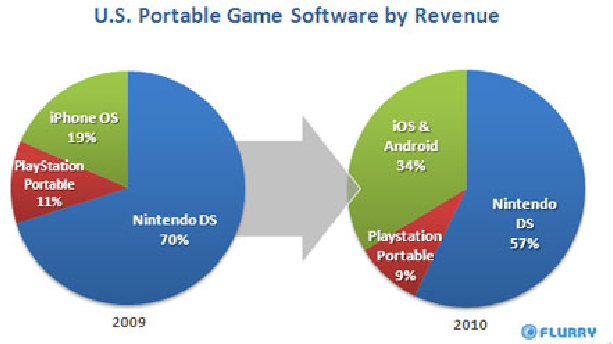
\includegraphics[scale=0.5]{img/marche_console_portable.png} \end{center}

%\begin{itemize} 
%		\item{Peu couteux}
%		\item{Grand nombre de mini-jeux et de jeux}
%		\item{Public visé plus large}
%\end{itemize}
\end{frame}


\subsection{Les sytèmes d'exploitations}


\begin{frame}
\frametitle{Présentation}
\framesubtitle{Android}

	\begin{minipage}{8cm}
		Le système d'exploitation possède : \\ 

	\begin{itemize} 
		\item Noyaux linux pour exploiter le matériel
		\item Librairies connues et open source (OpenGL ES, SQLite,...)
		\item Machine virtuelle Java (Dalvik virtual machine)
		\item API Java riche (package de Java SE, open source ou spécifique au système)
	\end{itemize}
	\end{minipage} 
	
\includegraphics[scale=0.2]{img/android.png} 

\end{frame}


 


\begin{frame}
\frametitle{Présentation}
\framesubtitle{Android}
	\begin{minipage}{8cm}
	Les possibilités de développement sont: \\ 

	\begin{itemize}
		\item Langage principal Java, développement en C/C++ possible
		\item Kit de développement multiplateforme
		\item Développement sur téléphone ou sur émulateur
		\item Déploiement des applications peu coûteux
	\end{itemize}
	\end{minipage}  
\includegraphics[scale=0.2]{img/android.png} 
\end{frame}


 


\begin{frame}
\frametitle{Présentation}
\framesubtitle{iOS}
	\begin{minipage}{8cm}
Le système d'exploitation possède : \\

	\begin{itemize} 
		\item Noyau dérivé de Mac OS X
		\item Librairies connues et open source (OpenGL ES, SQLite,...)
		\item Pas de machine virtuelle. Code compilé en C.
		\item API Objective-C riche (Core OS, Cocoa Touch,...)
	\end{itemize}
	\end{minipage}  
\includegraphics[scale=0.2]{img/apple.png} 
\end{frame}


 


\begin{frame}
\frametitle{Présentation}
\framesubtitle{iOS}
	\begin{minipage}{8cm}
	Les possibilités de développement sont: \\ 

	\begin{itemize}
		\item Langage principal Objective-C, développement en C possible
		\item Kit de développement disponible sur Mac OS seulement
		\item Développement sur emulateur seulement.
		\item Déploiement des applications coûteux
	\end{itemize}
	\end{minipage}  
\includegraphics[scale=0.2]{img/apple.png} 
\end{frame}


 
\subsection{Le jeu Bomberman}


\begin{frame}
\frametitle{Présentation}
\framesubtitle{Bomberman}
\begin{tabular}{cc}

\begin{minipage}{7cm}
Histoire
	\begin{itemize}
		\item Jeu d'action.
		\item Première apparition en 1987.
		\item Développé par Hudson Soft.
		\item Développé sur plusieurs consoles.
		\item Succès grâce au mode multijoueur sur certaines consoles.
	\end{itemize}
\end{minipage} 
&
\begin{minipage}{8cm}

\includegraphics[scale=0.3]{img/bomberman1.png} 
\end{minipage} 

\end{tabular}{cc}

\end{frame}


 


\begin{frame}
\frametitle{Présentation}
\framesubtitle{Bomberman}
	Principe : \\
	
	\begin{minipage}{5cm}
		\begin{itemize}
			\item Le joueur incarne un poseur de bombes.
			\item But du jeu: détruire ses ennemis.
		\end{itemize}
	\end{minipage}
	\begin{minipage}{5.5cm}
		\begin{itemize}
			\item Multiples bonus (Bonus de vie, de bombes, de vitesse,...).
			\item Multiples malus (Obligation de poser des bombes,...).
		\end{itemize}
	\end{minipage} 
	
	\begin{center}
		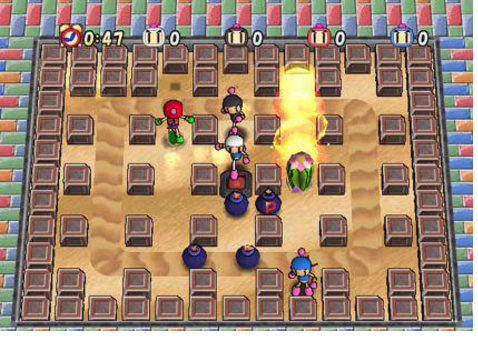
\includegraphics[scale=0.35]{img/bomberman2.png}
	\end{center}

\end{frame}


 
\subsection{Rapport avec l'enseignement}


\begin{frame}
\frametitle{Présentation}
\framesubtitle{Rapport avec l'enseignement} 
Ce TER nous a permis de mettre en application les connaissances acquises dans nos parcours d'enseignements. \\ $\,$ \\
	
\begin{tabular}{cc}
	 Aspect technique &  Aspect pédagogique \\ 
				     & 					  \\
	Intelligence artificelle & I2A \\
	Communication mobile-serveur & CASAR \\
	Serveur d'application & DIWEB \\
	Conception de logiciel & Génie Logiciel

\end{tabular}
	
\end{frame}



